\chapter{Robot Social Behaviour and Child Learning} \label{chap:socasoc}

\begin{framed}
	\textbf{Key points:}
	
	\begin{itemize}
	\item An experimental methodology was devised to teach and measure children's performance in prime number identification.
	\item `Social' and `asocial' robot conditions were derived from observation of a human tutor. These conditions were compared with a no-robot control, and a no-robot, no-lesson control.
	\item Children learn a significant amount from the robot, but not from the no-robot or no-lesson controls.
	\item However, children in the `asocial' robot condition learn a significant amount, whilst those in the `social' condition do not. Whilst initially surprising, \gls{nonverbalimm} ratings may provide an explanation for these differences.
	\end{itemize}
\end{framed}

Part of the work presented in this chapter has been published in \cite{kennedy2015robot}
\footnote{Note about technical contributions in this chapter: the author wrote original software for the touchscreen, replacing the software previously used from the \acrshort{alize} project. This new software (or a variation thereof) continues to be used in Chapters \ref{chap:nviexperiment} and \ref{chap:verbal}. The robot code was also upgraded from Urbi v2.7.5 to v3.0, this was performed in part by the author and in part by the \acrshort{alize} project. All high-level robot social behaviour programming was done by the author.}. The final publication is available from the ACM via:\newline http://dx.doi.org/10.1145/2696454.2696457


\newpage
The previous chapter explored the impact of robot embodiment on child \gls{learning}. No learning differences were observed, but this may have been a product of complications introduced by the novel dataset used. However, there were clear differences in the social behaviour of the children towards the physically present, real, robot. This bodes well for the use of robots in educational interactions, given the connection between social behaviour of this nature and \gls{learning} in the \acrshort{hhi} literature \citep{richmond2003development}.

The influence of social behaviour on \gls{learning} was explored in Chapter \ref{chap:background} from a mix of \acrshort{hhi} and \acrshort{hri} literature. It was established that between humans, social behaviour has a large impact on \gls{learning}. Both verbal \citep{gorham1988relationship} and non-verbal \citep{richmond2003development} aspects of behaviour can influence learning outcomes, with various guidelines presented for appropriate teaching behaviour. However, these guidelines are relatively broad and high-level, without specifically indicating certain aspects that social roboticists require for behavioural design. For example, \cite{richmond2003development} suggests that performing more gestures should lead to more positive \gls{learning} outcomes, but the specific type of gesture and timing of these gestures is not specified.

Research conducted in \acrshort{hri} has sought to confirm some of these observations from human studies, but with results at a greater degree of specificity as required for behavioural design \citep{huang2013modeling}. Other findings from \acrshort{hhi} literature have been confirmed with robots and adults, for example \cite{szafir2012pay}, but it remains to be seen as to whether these findings also translate to domains with children. The robot behaviour in this chapter is derived from a human model completing the \gls{learning} task with children so that an appropriate behaviour could be devised. The behaviour produced is then evaluate against an `inverse' to provide a counter to what is considered as an optimal social behaviour (assuming that a human is an optimal model for social behaviour).

This chapter seeks to not only explore the effect that the presence that a robot has on the interaction taking place, but to also assess how the behaviour that this robot employs influences child social responses and \gls{learning} outcomes. Whilst the previous chapter actively sought to avoid covering material included the school curriculum, this chapter instead places the work into the context of the curriculum. This is done to provide a clear relevance for the findings, and to maximise the chance of the children understanding why the subject is being taught (thereby improving their motivation to learn). Of course, this also requires prior ability to be more carefully controlled, but a novel topic within the curriculum is selected. The methodology is based on the teaching strategy used by teachers to provide further validity to the approach.

%%%%%%%%%%%%%%%%%%%%%%%%%%%%%%%%%%%%%%%%%%%%%%%%%%%%%%%%%%%
\section{Hypotheses}\label{sec:socasoc-hyp}
The aim for the study was to explore both embodiment and the social behaviour employed by a robot. It is useful to verify whether a robot brings benefits to the \gls{learning} in this specific context: a sorting task, using the NAO robot, with children, in addition to evaluating the impact of social behaviour on \gls{learning} (as a step towards establishing appropriate social behaviour for robots in such tasks). Prior work has suggested that the presence of a robot will result in greater learning gains \citep{han2005educational, leyzberg2012physical}; this drives the hypothesis for the embodiment differences (H1). Positive effects of social behaviour have been observed in other \acrshort{hri} studies such as \citet{leyzberg2014personalizing} and \citet{saerbeck2010expressive}, and psychology studies such as \citet{atkinson2005fostering} and \citet{mayer2004personalization}. These prior works are used as the basis for the hypothesis about social behaviour (H2). The hypotheses are as follows:
\begin{enumerate}
	\item[\textbf{H1}:] The presence of a robot will result in greater \gls{learning} gains than when a robot is not present given equal information content.
	\item[\textbf{H2}:] A robot with greater social skills will result in greater \gls{learning} gains than a counter social robot.
\end{enumerate}

%%%%%%%%%%%%%%%%%%%%%%%%%%%%%%%%%%%%%%%%%%%%%%%%%%%%%%%%%%%
\section{Experimental Setup}\label{sec:social-setup}
Four conditions are used in a between-subjects design to explore the social presence of a robot and the effect of social behaviour: 2 without a robot, and 2 using a robot with differences in the social behaviour. The methodology of the experiment was designed based on previous work with child \gls{learning} in sorting tasks, as in Chapter \ref{chap:embodiment}, and with sub-tasks leading to a combination of knowledge in a larger primary \gls{learning} objective, as in \citet{leyzberg2014personalizing}. The following section will detail the participants involved, the interaction scenario, the task structure, the robot behaviour and the conditions used in the experiment.

\subsection{Participants}\label{sec:socasoc-participants}
A total of 53 children had permission to take part in the study. Due to technical issues, 8 of the children's data had to be excluded, leaving 45 children included in the study (23F, 22M). All participants were aged 7 or 8 and from the same year group at a primary school in the U.K. Participants were randomly distributed between conditions, whilst maintaining a balance of gender and mathematics ability (based on their teacher's assessment) between the groups. For the split between conditions, please see Section~\ref{sec:socasoc-conds}. Those in the robot conditions were requested for permission to film, which was granted in all but 2 of the cases. One video had to be excluded from analysis as it was not possible to see the child's eyes. Therefore, video analysis was conducted on 20 interactions.

\subsection{Interaction Scenario}\label{sec:socasoc-scenario}
Interactions took place either in an unused classroom, or a relatively quiet public space in a primary school in the United Kingdom. The child was brought into the experiment area and would be sat facing a robot, an Aldebaran Nao, with a 27 inch touchscreen horizontally between them (Figure~\ref{fig:ch7_schem}). A Microsoft Kinect was placed above and behind the robot to track the child's face. Two video cameras were also positioned around the setup: one to record the child's face and actions and another to record the robot's actions. The use of a touchscreen mediator \citep{baxter2012touchscreen} allows a consistent, constrained environment, so the robot's social behaviour can be manipulated without impacting on the nature of the task or the content of the \gls{learning} \citep{kennedy2013constraining}.

\begin{figure}[t!]
    \centering
    \includegraphics[width=0.6\textwidth]{images/ch7_schematic_compressed.pdf}
    \caption{Schematic overview of the interactions under investigation in this paper. Two interactants (the child and the robot) face one another over the touchscreen. Two video cameras record the interactants during the studies. A Microsoft Kinect tracks the child's face. Two experimenters are in the room, but out of view of the child. Figure not to scale.}
    \label{fig:ch7_schem}
\end{figure}

The \gls{learning} content for the interaction was devised with the help of primary school teachers from a different school to the one where the study took place. The aim was to select a topic with which children had no prior exposure, but could be learnt in a relatively short time. Prime numbers were determined to be an ideal solution. Calculation of whether a number is prime can be performed by using division (for more detail see Section \ref{sec:socasoc-taskstruct}). Children of the age used in the study are familiar with division, but have not been taught what a prime number is at this stage of their education. The study was conducted at the end of an academic year. The children would typically learn about prime numbers in the following academic year, which would only be 3 months later. As such, the concepts involved, and difficulty of the task, are suitable for children at this developmental stage. The experimental context is also more relevant to the school curriculum, which offers the findings greater veracity.

The touchscreen presents different numbers for sorting. The child can touch the numbers to drag and drop them into categories. An example library here would display text labels at opposite sides of the screen, such as `prime' and `not prime', with some numbers in between (Figure~\ref{fig:ch7_task}). The child can touch these numbers and drag them to the label for categorisation. The touchscreen sends all state information to the robot so that the robot knows the child's moves, and the robot can make moves itself by synchronising movement with on-screen animation (the robot does not physically touch the screen; \citealp{baxter2012touchscreen}).

\begin{figure}[t!]
    \centering
    \includegraphics[width=0.7\textwidth]{images/ch7_pretest.png}
    \caption{Example of the sorting task used. This is a screenshot of one of the tests used in the experiment. Children can touch a number, drag it over the `prime' or `not prime' label and release to make a categorisation. The number will then shrink and move into the boxes beside the category label.}
    \label{fig:ch7_task}
\end{figure}

\subsubsection{Task Structure}\label{sec:socasoc-taskstruct}
The structure for the task was created partly through necessity for measuring \gls{learning} and partly through a logical method of calculating primes known as the Sieve of Eratosthenes \citep{oneill2009sieve}. The Sieve of Eratosthenes works through a group of numbers, eliminating non-prime numbers in a methodical manner to leave only the prime numbers. For the number range used in this study all composites can be eliminated by dividing by 2, 3, 5 and then 7.

\begin{figure}[t!]
    \centering
    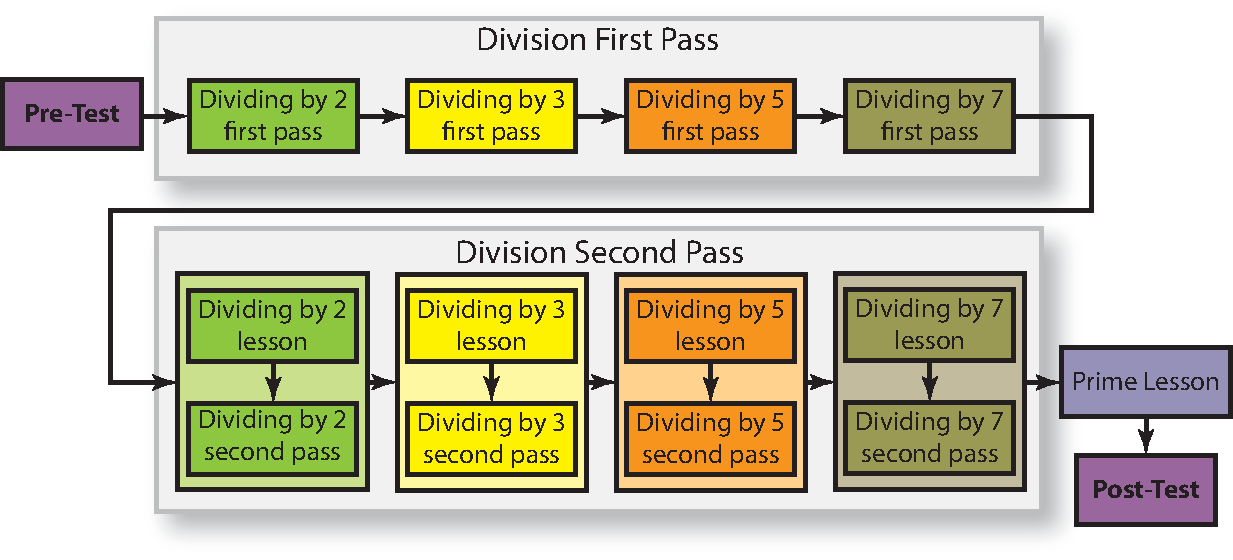
\includegraphics[width=1.0\textwidth]{images/ch7_task_structure.pdf}
    \caption{Structure of the task used in the interactions, showing robot lesson positions.}
    \label{fig:ch7_structure}
\end{figure}

The task was structured so that appropriate measures could be taken for both prime number \gls{learning} and division learning. Additionally, the task structure allows the examination of the children's division skills prior to the prime number post-test, which is important as these division skills are necessary for the calculation of primes (Figure~\ref{fig:ch7_structure}).

Pre- and post-tests each consisted of 12 numbers being presented on screen; 6 were prime and 6 were non-prime (Figure~\ref{fig:ch7_task} shows an example test). Both tests avoided numbers from the prime lesson and had balanced distributions of numbers across the range being used (10-70).

Each practice library in the division `pass one' consisted of 8 examples - 4 of which could be divided with no integer remainder by the number in question, and 4 which could not. This first pass was used to obtain a measurement for each child in how well they could divide by each of the divisors required for the main goal of calculating prime numbers. The number of examples in division `pass two' totalled 24, but the distribution between each of the 4 divisors (2, 3, 5 and 7) was dependent upon the condition and performance in pass one (see Section \ref{sec:socasoc-conditions}).

\subsubsection{Lesson Content}\label{sec:socasoc-lessons}
In the second division pass, a lesson was provided for each of the divisors: 2, 3, 5 and 7. This involved verbal instructions and categorisations on-screen. Each lesson consisted of a short verbal overview of the technique, followed by categorisation of 2 examples with verbal narration explaining the application of the technique to the examples. One example could be divided with no remainder, and the other could not. The lessons were not to teach the concept of the division, but often to provide a `trick' whereby the division could be accomplished more easily. The lessons were explanations of the following concepts:
\begin{itemize}
	\item Divisible by 2 - the number is even (ends in 0, 2, 4, 6 or 8)
	\item Divisible by 3 - sum the digits of the number and test if that divides by 3
	\item Divisible by 5 - the number ends in 0 or 5
	\item Divisible by 7 - no trick available; a reminder that a number in the 7 times table will be divisible by 7
\end{itemize}

The lesson about primes which took place after the second division pass used the information from the earlier division lessons to draw together the practice the child had with dividing by 2, 3, 5 and 7 into calculating whether numbers were prime. The concept of primes was explained (a number divisible, with no remainder, by only 1 and itself) before two worked examples were completed on-screen - one prime and one not prime. The Sieve of Eratosthenes was adapted to eliminate numbers one-by-one for categorisation. Children were instructed to consider each number to be categorised in turn, attempting to divide it by 2, 3, 5 and 7. If the number divided by any of these then it was not prime, otherwise it was prime.

\begin{figure*}[t!]
    \centering
    \includegraphics[width=1.0\textwidth]{images/ch7_snapshots_small_compressed.pdf}
    \caption{Snapshots taken from the video recordings of interactions. Both the social (\textit{left}, looking at the child) and asocial robot (\textit{right}, actively avoiding the gaze of the child) conditions are pictured to show the difference in gaze behaviour between them.}
    \label{fig:ch7_conditionsnaps}
\end{figure*}

\subsection{Conditions}\label{sec:socasoc-conds}
In order to address the hypotheses, four conditions were devised. The `division only' condition is used to provide the manipulation check;  it is useful to verify that the lessons provided do indeed facilitate learning, with no robot present. The `asocial non-personalised robot' condition described below provides an overlap between the embodiment and social behaviour research questions. The content is identical to the `screen only' condition, thereby providing the comparison for physical embodiment. The `social personalised robot' condition is then used as a contrast in terms of social behaviour.
\begin{enumerate}
	\item \textbf{Division only} [\textit{n}=11] - division pass one, followed by division pass two without any lessons. Conducted on the touchscreen only, with no robot present.
	\item \textbf{Screen only} [\textit{n}=11] - the full interaction as described in Section \ref{sec:socasoc-taskstruct}, but with no robot present. All feedback and lesson content is delivered by the speakers in the screen.
	\item \textbf{Asocial non-personalised robot} [\textit{n}=11] - identical script to the `screen only' condition, but with the robot delivering the content. All verbal content and feedback is given by the robot; the screen now only displays the numbers for the task. Robot behaviour is designed to be non-social (see Section \ref{sec:socasoc-robbehave} for full details).
	\item \textbf{Social personalised robot} [\textit{n}=12] - a social version of the full interaction. All lesson content is kept the same as the asocial robot condition, but the non-lesson speech is adjusted to be more social. Robot non-verbal behaviour is also designed to be social.
\end{enumerate}

\subsection{Robot Behaviour}\label{sec:socasoc-robbehave}
Human tutors are known to be effective, using social behaviour and adapting to the \gls{learning} needs of the child. As such, the social robot behaviour was based on a human tutor's behaviour when taking five children through the task on the touchscreen. Section \ref{sec:socasoc-conditions} outlines four observed behavioural dimensions that were implemented on the robot. Whilst maintaining balance between the conditions, the inverse for each dimension is used for the asocial robot behaviour in order to evaluate Hypothesis~2.

The phrases and actions used by the human were observed and implemented in the social robot model. It is posited that behaviour is perceived by the child as an integration of cues \citep{zaki2013cue}, meaning that each dimension must be considered in context of the others. Consequently, personalisation and social behaviour are considered inseparable in assessing Hypothesis~2 for this study, following the human model.

\subsubsection{Condition Independent Behaviour}
Both robot conditions adopted the following basic behaviour during the image categorisation portions of the task:

\textit{Move Suggestions} - During each stage of the interaction, if the child was hesitant in making moves then the robot would move a number to the centre of the screen and suggest that the child work on that number next. The decision about when to move was probabilistic and cued by the child's behaviour. If the child did not make a categorisation for 6 seconds, then there was a 25\% chance that the robot would move, with the decision repeated every 2 seconds until a move was made - the 6 second timer would then start again.

\textit{Categorisation Feedback} - The robot would provide verbal feedback on the child's categorisations. Not every categorisation received feedback; there was a 25\% chance of feedback on each categorisation - following the human tutor model.

\subsubsection{Robot Condition Differences}\label{sec:socasoc-conditions}
\textit{Verbal Content} - The script for the social robot speech was taken from the human tutor; this was then modified for the asocial robot by removing any personalisation, i.e., ``Johnny, we'll do dividing by 2 next'' becomes ``You'll do dividing by 2 next''. The total amount of speech was kept as close as possible between the conditions, and the lesson content was the same.

When providing speech alongside a suggestion, or when providing feedback, a number of phrases were available and selected at random. The asocial robot had only 2 options for each event (compared to the social robot's 8), thereby making it very repetitive.

\textit{Gestures} - The social robot script used for the introduction and some of the lessons included iconic gestures. In the asocial condition, these were placed at inappropriate times, for example, the robot would wave its arm to greet the child half way through a sentence, rather than when it says hello at the start. The same gestures were used in both conditions, the only difference was their position in the script.

\textit{Personalisation} - The social robot would use the child's name in greeting, just before the post-test and in the goodbye script. The asocial robot would not use the child's name at all. Personalisation of \gls{learning} content was also provided by the social robot. 

The performance of the child in the first division pass would dictate how many examples of each division library they would do in the second pass. A total of 24 numbers were always used in the second division pass. For the asocial condition, these were split equally between divisors, so 6 numbers for each of dividing by 2, 3, 5 and 7. In the social condition a minimum of 3 numbers were used per divisor, but the remaining 12 numbers were distributed between the divisors based on how many of each divisor the child got wrong in the first pass. Therefore, they had more practice on numbers that they were weaker at in the second pass.

In the second division pass, for each divisor library, there was also a reminder of the lesson available. In the asocial condition, this reminder would be delivered by the robot half way through the categorisations for that library (i.e., after the 3rd of the 6 categorisations to be made). In the social condition, the reminder was given after the first incorrectly categorised image.

\textit{Gaze} - The social robot gaze was constrained so that it would generally be looking towards the touchscreen or in the direction of the child. Additionally, a Microsoft Kinect was used for tracking the child's head pose. If the child's head pose was directed towards the robot, then the robot would respond by looking back at the child. In the asocial condition, the robot was intentionally programmed to look up and to the side so that the gaze would avoid the child (Figure~\ref{fig:ch7_conditionsnaps}).

\subsection{Procedure}\label{sec:socasoc-wizard}
One of the experimenters shown in Figure~\ref{fig:ch7_schem} controlled the start and end of the autonomous behaviour. This individual had three responsibilities: \textit{1)} to type in the name of the child for the social robot condition before the child arrived in the room, \textit{2)} to click a button once the child was sat down in front of the robot to denote the start of the interaction, and \textit{3)} to click an `emergency' button if anything went wrong, where the robot would gracefully end the interaction. All other robot behaviour was fully autonomous.

%%%%%%%%%%%%%%%%%%%%%%%%%%%%%%%%%%%%%%%%%%%%%%%%%%%%%%%%%%%
\section{Results}\label{sec:social-results}
This section will present the results from each of the conditions in relation to the hypotheses. Learning will be considered either between the pre-and post-test improvements, or for division, between the total percent correct in division pass one and division pass two. The behavioural analysis is derived from video coding of the child's gaze as previous work has highlighted gaze as the primary behaviour of interest in interactions of this nature \citep{kennedy2015comparing}. The video coding was completed by one coder for all videos. Coding was verified by second-coding 20\% of the videos, as in \cite{moshkina2014social}, with an average Cohen's Kappa of 0.80 signifying substantial agreement \citep{landis1977measurement}.

The conditions were split to have an equal balance of ability based on an estimate by the children's teacher (higher, middle and lower tiers). Comparing the approximate ability level of the children that was provided by their teacher against their performance in the first division pass (at which point they've had no lesson input), Pearson's \textit{r} correlation is 0.638. This is a good correlation, which confirms that the teacher's estimate is reflected in the results of this study and therefore that the conditions are balanced for ability.

The mean average length of the interactions were: 974s (95\% CI [750s,1199s]) in the asocial robot condition, 1011s (95\% CI [786s,1236s]) in the social robot condition, and 873s (95\% CI [680s,1066s]) in the screen only condition. The average length of the division only condition (\textit{M}=452s, 95\% CI [277s,629s]) was much shorter as the robot lessons, pre-test and post-test add a lot of time.

\subsection{Learning from Lessons}\label{sec:socasoc-results-division}
A 2 tailed, unpaired \textit{t}-test was conducted to compare the improvement between division pass one and division pass two in the division only (no lessons) and screen only (with lessons) conditions (with no robot present). The groups were used with independence of observations, and a continuous measure. Distributions did not significantly deviate from normality (Kolmogorov-Smirnov test; $\textit{p}>.05$) and had homogeneity of variances (Levene's test; $\textit{p}>.05$). There was a significant difference in the scores for division only (\textit{M}=5.40, 95\% CI [1.17,9.63]) and screen only (\textit{M}=14.68, 95\% CI [10.65,18.71]) conditions; \textit{t}(20)=3.114, \textit{p}=.006 (Figure~\ref{fig:ch7_divisionimprove}). This manipulation check shows that the improvement was significantly higher when the lessons were present. The result here is not surprising, but it is beneficial to show the effectiveness of the division lessons.

\begin{figure}[t!]
    \centering
    \includegraphics[width=0.6\textwidth]{images/ch7_division_improvement.pdf}
    \caption{Improvement between division pass one and division pass two in percent for the division only and screen only conditions. Significantly greater improvement occurred in the `screen only' condition (where division lessons were present) when compared to the `division only' condition (where division lessons were not present), indicating that the lessons have a significant, positive impact on child division. \textit{Error bars} show 95\% Confidence Interval, ** indicates significance at the \textit{p}\textless .01 level.}
    \label{fig:ch7_divisionimprove}
\end{figure}

\subsection{Robot Presence}\label{sec:socasoc-results-robot}
To examine how the robot affects the \gls{learning} of the child, the improvement from pre-test to post-test scores was compared between the screen only and (combined) robot conditions. All pre-test and post-test scores are out of 12. None of the children who took part in the study reported to know what a prime number was before the interaction. As a result, based on 2 options for each categorisation, it would be expected that the pre-test scores would be around chance (50\% out of 12 correct). Pre- and post-tests are paired observations, on a continuous measure, with distributions that did not significantly deviate from normality (Kolmogorov-Smirnov test; $\textit{p}>.05$), so paired samples \textit{t}-tests are used for their analysis. Unpaired \textit{t}-tests are used to compare between robot conditions as the observations are then independent.

In the screen only condition a 2 tailed, paired \textit{t}-test reveals no significant difference between the scores for the pre-test (\textit{M}=5.91, 95\% CI [4.68,7.13]) and post-test (\textit{M}=7.36, 95\% CI [5.49,9.24]); \textit{t}(10)=1.027, \textit{p}=.329. However, when a robot is present there is a significant difference in scores between the pre-test (\textit{M}=6.04, 95\% CI [5.15,6.94]) and the post-test (\textit{M}=7.78, 95\% CI [6.61,8.95]); \textit{t}(22)=2.997, \textit{p}=.007. To further explore this result, the screen only pre-test and post-test scores were compared with those in the asocial robot condition. These two conditions are identical in the script that is used (the screen plays recorded clips of the robot voice) and the lack of personalisation. For the asocial robot, the difference is significant when the same test is run between scores for the pre-test (\textit{M}=6.27, 95\% CI [5.00,7.54]) and post-test (\textit{M}=8.45, 95\% CI [6.84,10.07]); \textit{t}(10)=2.597, \textit{p}=.027. However, it should be noted that there was no significant difference in the improvement between the screen only (\textit{M}=1.46, 95\% CI [-1.32,4.23]) and asocial robot (\textit{M}=2.18, 95\% CI [0.54,3.83]) conditions; \textit{t}(20)=0.442, \textit{p}=.664, when using a 2 tailed, unpaired \textit{t}-test. Despite the asocial robot leading to significant learning gains and the screen only condition not, the lack of significant difference between the conditions means that there is no conclusive statistical evidence for learning improvement due to the robot. This means that Hypothesis 1 is not supported: the learning gains were indeed greater when a physical robot was present, but this difference was not statistically significant.

\subsection{Social Condition}\label{sec:socasoc-results-social}
As shown in the previous section, the \gls{learning} gains for the asocial robot were significant. When conducting a 2 tailed, paired \textit{t}-test for the social robot condition there is no significant difference between the pre-test (\textit{M}=5.83, 95\% CI [4.54,7.13]) and post-test (\textit{M}=7.17, 95\% CI [5.50,8.84]); \textit{t}(11)=1.627, \textit{p}=.132. Whilst all conditions show improvement between the pre-test and the post-test, the only condition where the \gls{learning} gain is significant is with the asocial robot; both the social robot and screen only conditions show non-significant improvement (Figure~\ref{fig:ch7_prepostgraph}). This result contradicts Hypothesis 2, that a more social robot will result in greater \gls{learning} gains than a less social robot.

\begin{figure}[t!]
    \centering
    \includegraphics[width=0.7\textwidth]{images/ch7_pre_post_graph.pdf}
    \caption{Pre-test and post-test scores for the asocial robot, social robot and screen only conditions. \textit{Error bars} show 95\% Confidence Interval, * indicates significance at the \textit{p}\textless .05 level.}
    \label{fig:ch7_prepostgraph}
\end{figure}

To explore the impact that the \gls{learning} personalisation may have had on the results, the lesson reminders and practice of numbers in the second division pass are considered. In the asocial condition a reminder of the lesson is given for each divisor, whereas in the social condition, reminders are only given when the child makes a mistake. This meant that in the asocial condition a total of 44 reminders were given (\textit{M}=4.00 per interaction; no deviation), whereas in the social condition a total of 22 reminders are delivered (\textit{M}=1.83, 95\% CI [0.94,2.73] per interaction). This is not surprising, as most children can comfortably divide by 2 and 5 at this age; thereby eliminating the need for around half of the reminders. When correlating the number of reminders provided to children in the social robot condition with their improvement between pre- and post-test score, Pearson's correlation \textit{r}(10)=-0.418, \textit{p}=.176. This is a moderate negative correlation, which suggests that receiving fewer reminders does not reduce the child's performance.

Additionally, children in the social robot condition were given the opportunity to practice more of the numbers that they were weaker at (following the human model described in Section \ref{sec:socasoc-robbehave}). There is a possibility that this could have been a de-motivator if they then performed poorly in this phase of the interaction. However, this seems unlikely as it is found that there is no significant difference between the performance in the second division pass between children in the social condition (\textit{M}=82\% correct, 95\% CI [71\%,93\%]) and those in the asocial condition (\textit{M}=85\% correct, 95\% CI [75\%,95\%]); \textit{t}(21)=0.432, \textit{p}=.670.

In order to investigate the reasons behind why children's \gls{learning} gains are not as great when the robot is social compared to when it is asocial, the children's behaviour and self-reported view of the robot were analysed. From video coding of the interactions, it was found that children look significantly more often at the social robot (\textit{M}=12.9, 95\% CI [10.4,15.3]) than at the asocial robot (\textit{M}=8.9, 95\% CI [6.9,10.9]); \textit{t}(18)=2.425, \textit{p}=.026 (Figure~\ref{fig:ch7_gazeatrobot}). Values are provided in seconds of gaze at the robot per minute of interaction; this normalisation allows for comparison across interactions of different lengths.

\begin{figure}[t!]
    \centering
    \includegraphics[width=0.7\textwidth]{images/ch7_gaze_at_robot.pdf}
    \caption{Child gaze towards the robot in seconds per minute, split by robot condition. \textit{Error bars} show 95\% Confidence Interval, * indicates significance at the \textit{p}\textless .05 level.}
    \label{fig:ch7_gazeatrobot}
\end{figure}

The children completed a pre-questionnaire and a post-questionnaire before and after the interaction. These were very short, with just 4 questions in the pre-questionnaire and 2 questions for the post-questionnaire. The questionnaires were used to see what the children expected from the interactions, and subsequently how they viewed the robot afterwards. Despite being told by the experimenters several times before their interactions that they would be \textit{taught} by a robot \textit{teacher}, with the robot script emphasising this point too, the children in the social robot condition consistently reported that they thought the robot was a `friend' after the interaction. The question asked ``For me, I think the robot was like a -'' with 8 options available: brother or sister, classmate, stranger, relative (e.g., cousin or aunt), friend, parent, teacher, and neighbour.

It was expected that the children would report the robot to be a teacher (as this is what they had been told), so their responses were grouped into either `teacher' or `not teacher'. In the social condition, 17\% of the children reported the robot to have been like a teacher, compared to 64\% in the asocial condition. As the data consists of two groups of categorical data, Fisher's exact test is used to show that the responses differ significantly by condition, \textit{p}=.036 (Figure~\ref{fig:ch7_questionnaire}).

\begin{figure}[t!]
    \centering
    \includegraphics[width=0.7\textwidth]{images/ch7_quest_graph.pdf}
    \caption{Post-questionnaire responses of the children when asked what they thought the robot was like. Eight options, including `teacher' were available.}
    \label{fig:ch7_questionnaire}
\end{figure}

It is clear from the children's gaze and self-reported responses that the difference in robot behaviour between conditions has an effect on the children's behaviour and attitudes towards the robot. It is suggested that these differences could account for the difference in \gls{learning} gains observed between the social and asocial robot conditions. Whilst the robot is providing the lesson about prime numbers, it demonstrates two examples on the screen by highlighting the numbers, discussing them and correctly categorising them. Therefore, during this period it is useful to look at the screen. During the prime lesson the average amount of gaze towards the social robot (\textit{M}=26.9 secs/min, 95\% CI [22.9,30.9]) is significantly higher than the gaze towards the asocial robot (\textit{M}=17.0 secs/min, 95\% CI [11.0,23.1]); \textit{t}(18)=2.669, \textit{p}=.016 (unpaired \textit{t}-test). It is suggested that the additional attention directed towards the social robot's behaviour could distract the children from the content that it is delivering; this possibility is further discussed below (Section~\ref{sec:social-discussion}).

%%%%%%%%%%%%%%%%%%%%%%%%%%%%%%%%%%%%%%%%%%%%%%%%%%%%%%%%%%%
\section{Discussion}\label{sec:social-discussion}
From the analysis of the results it is clear that the lessons for division have a positive effect on the children's performance. This validates part of the teaching behaviour and demonstrates that the children have the ability to understand the robot's voice and apply knowledge gained from the lessons in the task on-screen.

When the asocial robot is present, despite having the same content as the screen only condition, the improvement between pre-test and post-test is significant. This is a demonstration of the social presence effect; the addition of an agent into the interaction leads to improvement in task performance (although non-significant in this case), as observed before in other contexts, for example \citet{kose2009effects} and \citet{leyzberg2012physical}. However, the improvement is lost when the robot behaviour is changed to become more social. This is a surprising result, which contradicts both Hypotheses 1 (that a robot will provide greater \gls{learning} gains than the screen alone) and 2 (that a more social robot will result in improved \gls{learning} gains).

This result is in contrast to existing studies in the literature that Hypothesis 2 was based on. As described in Section~\ref{sec:socasoc-robbehave}, the robot behaviour was derived directly from that of a human tutor. This necessitates a perspective that integrates behavioural dimensions \citep{zaki2013cue} that emphasises sets of behavioural competencies (similar to the use by \citealt{saerbeck2010expressive}). This differs from the more typical focus on individual social cues, as in \citet{mayer2004personalization} and \citet{szafir2012pay}. With the interaction context (child-robot interactions in a school) and task content (learning mathematical concepts) also differentiating the work here from previous studies, this integrated cues perspective may merit further investigation in terms of the effects on the perceptions and performance of human interactants.

One factor that should be considered in the analysis of the results with regards to embodiment is the behaviour employed by the `screen only' condition. The `asocial robot' condition was used as the overlap between the embodiment and social behaviour research questions in this work. As such, the screen only condition used the same script as the asocial robot condition. This was done in part due to the personalisation aspects of the social robot condition; it was considered that the screen telling the child its name may be confusing given the lack of a visible character. The asocial robot condition did not contain these personalisation aspects, so was deemed a more appropriate choice. As a result, a comparison only between the screen only and asocial robot conditions can be made in terms of embodiment; a comparison with the social robot condition incurs a confound of social behaviour. Ideally, a 2x2 between-subjects design would have been used (i.e., through the addition of a `social screen' condition), but subject numbers were limited by class sizes, and a more thorough manipulation check would be required to understand how children perceived the social behaviour from the screen (particularly in light of the personalisation aspect). It could be the case that when the social skills variable is included in the design and the behaviour from the screen changes, different results would be observed.

One possible explanation for the unexpected findings with respect to \gls{learning} is that although the children looked at the social robot significantly more than the asocial robot during the lesson phase (which could be considered advantageous as the robot provides the lessons), they were paying attention to the social behaviour instead of the lesson content. An alternate explanation is that the social behaviour presented by the social robot places more cognitive load on the children, which may inhibit their capacity to process information related to the task \citep{sweller1994cognitive}. It may be that in the long-term, as the novelty of the social behaviour wears off, the social robot would then elicit better \gls{learning}, as indicated by \citet{kanda2004interactive}. However, further research is required to explore these ideas explicitly and in more detail.

\subsection{Child Perception and Ability}\label{sec:disc-ability}
In Section~\ref{sec:socasoc-results-social} it was shown that children in the asocial robot condition were more likely to report that they viewed the robot as a teacher than those in the social robot condition. The infrequency with which those in the social condition reported the robot to be like a teacher was surprising. The children were told several times before and during the interaction by both the robot and the experimenters that the robot was a teacher. It is suggested that there may be two reasons as to why this was the case. Firstly, it may be that the directness of the asocial robot conformed more to their expectations of what a robot teacher would be like than the social robot, which was less direct in its instructions. Secondly, the behaviour of the asocial robot may not have had enough character to change the children's perception of the robot as a teacher, whereas the social robot did. Unfortunately, no holistic measure was used to assess how the manipulation of the robot's social behaviour was perceived by the children. As such, it is not possible to evaluate whether the children saw either condition as more or less social. This limits the findings here as it is not possible to verify whether the differences in the child perceptions were directly linked to the social behaviour manipulation. It would additionally have been useful to verify that the children detected the differences between the robot social behaviour conditions. This is an aspect of the study design that is rectified in subsequent chapters. Interestingly, there was almost no correlation between the children's perception of the robot as a teacher and their performance; Pearson's \textit{r}(20)=-0.11, \textit{p}=.626.

There was only a weak correlation (Pearson's \textit{r}(20)=0.13, \textit{p}=.558) between the teacher-provided mathematics ability levels of the children and their subsequent improvement between pre-test and post-test. This is somewhat surprising, as one would expect the higher ability students to progress more given the same practice as those who were lower ability. This may highlight a limitation in the adaptiveness of the robot's behaviour used in this study. It is possible that a robot which is more adaptive could better respond to each individuals' needs and push them more effectively through the Zone of Proximal Development \citep{vygotsky1980mind}.

Due to the relatively small sample sizes used here, it only requires 2 or 3 subjects to perform particularly poorly or well to impact on the significance of the results. However, there is a trade-off between trying to carefully control the experiment and get greater subject numbers. Subjects were selected from the same school and year group so that they would have similar educational experiences and backgrounds. Due to limits on the sizes of school classes, it is likely that to get greater numbers would mean selecting subjects across multiple schools. This then introduces the risk of large variability between subjects' mathematical ability and the environment in which the experiment is conducted.

\subsection{Gender Differences}\label{sec:disc-gender}
One interesting aside that was noticed through additional exploratory analysis are differences between the genders. These results were not included in Section~\ref{sec:social-results} as they were not part of the original hypotheses for this study. However, as an interesting observation they have been included here, with the suggestion that they may be worth further research. A significant difference is found between the improvement between pre-test and post-test of girls (\textit{M}=2.77, 95\% CI [1.18,4.36]) and boys (\textit{M}=0.40, 95\% CI [-0.85,1.65]) when interacting with a robot present (both social and asocial conditions combined); \textit{t}(21)=2.192, \textit{p}=.040. These results show that the boys barely improved with a robot, whilst the girls improved quite substantially.

Additionally, girls who interacted with a robot present (\textit{M}=2.77, 95\% CI [1.18,4.36]) improved more than those without a robot present (\textit{M}=-0.40, 95\% CI [-3.71,2.91]). Whilst this difference is not quite significant (\textit{t}(16)=1.907, \textit{p}=.075), it seems as though there may be a possible trend. Gender differences due to social presence have been observed in other contexts in \acrshort{hri}, such as \citet{schermerhorn2008robot}, where females saw a robot as more machine-like. This could support the argument that the robot social behaviour distracts from the lesson content that it is delivering; girls, who may perceive the robot as less social, therefore outperformed the boys. Whilst there is not enough evidence here to make firm conclusions about this point, the effect of gender possibly merits more research in the context of educational interactions.

\subsection{Nonverbal Immediacy}\label{sec:ch7-disc-nvi}
The adult crowdsourced \gls{nonverbalimm} ratings of the robot behaviour provide further insight as to why the anticipated \gls{learning} differences were not found. 30 ratings of the `asocial' robot, and 33 of the `social' were acquired (for demographic details please see Appendix~\ref{app:crowdsourced}). The asocial robot received an average \gls{nonverbalimm} score of \textit{M}=48.5 (95\% CI [46.1,50.8]), with the social \textit{M}=49.0 (95\% CI [47.6,50.4]). These scores are not found to be significantly different when using an independent samples, two-tailed \textit{t}-test; \textit{t}(61)=0.372, \textit{p}=.711. At first glance, this is a surprising lack of difference, however, this is likely due to the way in which the \gls{nonverbalimm} questionnaire quantifies social behaviour. It does not take into account all aspects of interaction (as discussed in Chapter~\ref{chap:validation}), but just the quantity of overt nonverbal cues used. As the manipulation in this study was largely concerned with timing and verbal phrasing differences, these would not be picked up in the \gls{nonverbalimm} measure.

Section \ref{sec:disc-ability} showed that there were clear differences in the perception of the robot by children, but these differences are not reflected in the \gls{nonverbalimm} scores as rated by adults. Nevertheless, the correlation between \gls{nonverbalimm} and cognitive \gls{learning} gains would hypothesise no \gls{learning} differences between the conditions here, given the near-identical \gls{nonverbalimm} scores. To further explore this relationship in interaction-based \acrshort{hri} scenarios it would be useful to intentionally create and compare robot conditions with more contrasting \gls{nonverbalimm} behaviours.

%%%%%%%%%%%%%%%%%%%%%%%%%%%%%%%%%%%%%%%%%%%%%%%%%%%%%%%%%%%
\section{Summary}\label{sec:social-summary}
As expected, the use of lessons improved the children's performance between the first division pass and the second division pass, as shown in Section~\ref{sec:socasoc-results-division}. Partial evidence was found in support of the social presence effect. Section \ref{sec:socasoc-results-robot} showed that when a robot delivered the lessons to the child, the \gls{learning} was significant, whereas when the same information was provided by just a screen, without a robot, it was not, but the difference between the conditions was not statistically significant. By further breaking down the robot results into the two different behavioural conditions, it was found that the \gls{learning} remains significant with the asocial robot, where the script is identical to the condition without the robot present (where the \gls{learning} was not significant). However, these positive effects were not maintained when the robot was more social.

The results here have shown that a robot which is not appropriately social led to greater \gls{learning} gains of children in a maths task than a robot with appropriate social behaviours. This result contradicts expectations and predications made based on other studies in the literature (for example \citealp{mayer2004personalization} and \citealp{saerbeck2010expressive}). It is hypothesised that the social behaviour of the socially appropriate robot may distract from the content it is delivering with regards to the \gls{learning} task, whilst the asocial robot leads to disinterest, and therefore less distraction from the \gls{learning} task. Gaze behaviour of the children throughout the interaction and specifically during the prime numbers lesson is used to provide evidence for this suggestion.